\hypertarget{bin_2bbssp_8c}{
\section{bin/bbssp.c File Reference}
\label{bin_2bbssp_8c}\index{bin/bbssp.c@{bin/bbssp.c}}
}
Bottleneck Biconnected Spanning Subgraph solver. 

{\tt \#include \char`\"{}arrow.h\char`\"{}}\par
{\tt \#include $<$getopt.h$>$}\par


Include dependency graph for bbssp.c:\nopagebreak
\begin{figure}[H]
\begin{center}
\leavevmode
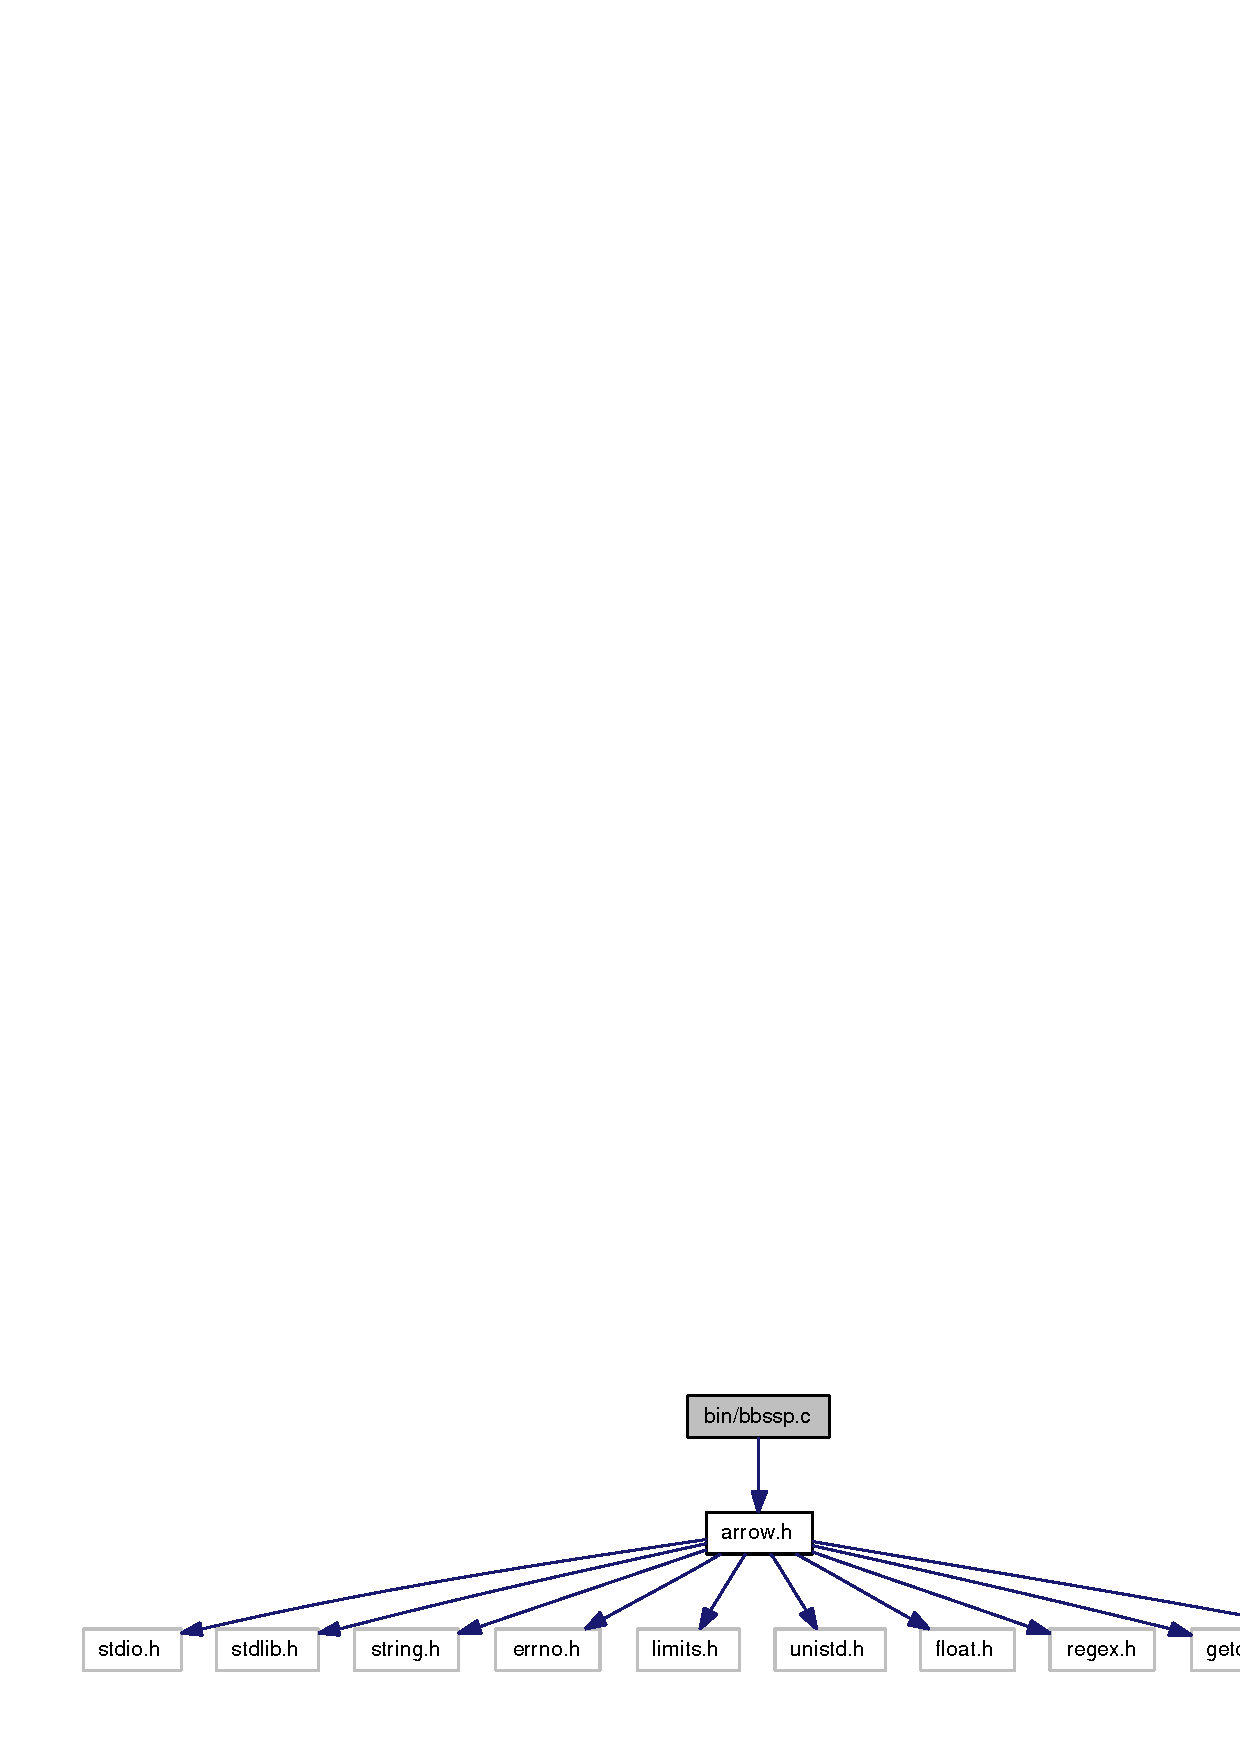
\includegraphics[width=257pt]{bin_2bbssp_8c__incl}
\end{center}
\end{figure}
\subsection*{Functions}
\begin{CompactItemize}
\item 
void \hyperlink{bin_2bbssp_8c_853216ac51aa181669ff4d3de74058a7}{print\_\-help} ()
\begin{CompactList}\small\item\em Prints help/usage message. \item\end{CompactList}\item 
void \hyperlink{bin_2bbssp_8c_6302aaae12249e8ea16bfdc7de892f21}{print\_\-version} ()
\begin{CompactList}\small\item\em Prints version message. \item\end{CompactList}\item 
void \hyperlink{bin_2bbssp_8c_e5ad5cbeccaedc03a48d3c7eaa803e79}{print\_\-usage} ()
\begin{CompactList}\small\item\em Prints usage message. \item\end{CompactList}\item 
void \hyperlink{bin_2bbssp_8c_72d0810dad1a2062df342005c15106b9}{read\_\-args} (int argc, char $\ast$argv\mbox{[}$\,$\mbox{]})
\begin{CompactList}\small\item\em Reads program arguments. \item\end{CompactList}\item 
void \hyperlink{bin_2bbssp_8c_f8424468968336a39cad523e50f3b65a}{print\_\-xml\_\-output} (int obj\_\-value, double total\_\-time, int argc, char $\ast$argv\mbox{[}$\,$\mbox{]})
\begin{CompactList}\small\item\em Prints output in XML format. \item\end{CompactList}\item 
int \hyperlink{bin_2bbssp_8c_0ddf1224851353fc92bfbff6f499fa97}{main} (int argc, char $\ast$argv\mbox{[}$\,$\mbox{]})
\end{CompactItemize}
\subsection*{Variables}
\begin{CompactItemize}
\item 
char $\ast$ \hyperlink{bin_2bbssp_8c_289c5900d90626d909f0a85d5a0ed61d}{program\_\-name}
\item 
char $\ast$ \hyperlink{bin_2bbssp_8c_a4f3a15de34c409bdec6ceacf93078ed}{input\_\-file}
\item 
int \hyperlink{bin_2bbssp_8c_78435df485756d3c16e77edcd8f6b938}{xml\_\-output} = ARROW\_\-FALSE
\end{CompactItemize}


\subsection{Detailed Description}
Bottleneck Biconnected Spanning Subgraph solver. 

Solves the bottleneck biconnected spanning subgraph problem (BBSSP) problem on the given input files.

\begin{Desc}
\item[Author:]John LaRusic \end{Desc}


Definition in file \hyperlink{bin_2bbssp_8c-source}{bbssp.c}.

\subsection{Function Documentation}
\hypertarget{bin_2bbssp_8c_0ddf1224851353fc92bfbff6f499fa97}{
\index{bin/bbssp.c@{bin/bbssp.c}!main@{main}}
\index{main@{main}!bin/bbssp.c@{bin/bbssp.c}}
\subsubsection{\setlength{\rightskip}{0pt plus 5cm}int main (int {\em argc}, \/  char $\ast$ {\em argv}\mbox{[}$\,$\mbox{]})}}
\label{bin_2bbssp_8c_0ddf1224851353fc92bfbff6f499fa97}




Definition at line 52 of file bbssp.c.

References arrow\_\-bbssp\_\-solve(), ARROW\_\-DEV\_\-NULL, arrow\_\-print\_\-error, arrow\_\-problem\_\-destruct(), arrow\_\-problem\_\-info\_\-destruct(), arrow\_\-problem\_\-info\_\-get(), arrow\_\-problem\_\-read(), arrow\_\-util\_\-redirect\_\-stdout\_\-to\_\-file(), arrow\_\-util\_\-restore\_\-stdout(), input\_\-file, arrow\_\-bbssp\_\-result::obj\_\-value, print\_\-xml\_\-output(), program\_\-name, read\_\-args(), arrow\_\-bbssp\_\-result::total\_\-time, and xml\_\-output.\hypertarget{bin_2bbssp_8c_853216ac51aa181669ff4d3de74058a7}{
\index{bin/bbssp.c@{bin/bbssp.c}!print\_\-help@{print\_\-help}}
\index{print\_\-help@{print\_\-help}!bin/bbssp.c@{bin/bbssp.c}}
\subsubsection{\setlength{\rightskip}{0pt plus 5cm}void print\_\-help ()}}
\label{bin_2bbssp_8c_853216ac51aa181669ff4d3de74058a7}


Prints help/usage message. 



Definition at line 100 of file bbssp.c.

References print\_\-usage(), and program\_\-name.

Referenced by read\_\-args().\hypertarget{bin_2bbssp_8c_e5ad5cbeccaedc03a48d3c7eaa803e79}{
\index{bin/bbssp.c@{bin/bbssp.c}!print\_\-usage@{print\_\-usage}}
\index{print\_\-usage@{print\_\-usage}!bin/bbssp.c@{bin/bbssp.c}}
\subsubsection{\setlength{\rightskip}{0pt plus 5cm}void print\_\-usage ()}}
\label{bin_2bbssp_8c_e5ad5cbeccaedc03a48d3c7eaa803e79}


Prints usage message. 



Definition at line 131 of file bbssp.c.

References program\_\-name.

Referenced by print\_\-help(), and read\_\-args().\hypertarget{bin_2bbssp_8c_6302aaae12249e8ea16bfdc7de892f21}{
\index{bin/bbssp.c@{bin/bbssp.c}!print\_\-version@{print\_\-version}}
\index{print\_\-version@{print\_\-version}!bin/bbssp.c@{bin/bbssp.c}}
\subsubsection{\setlength{\rightskip}{0pt plus 5cm}void print\_\-version ()}}
\label{bin_2bbssp_8c_6302aaae12249e8ea16bfdc7de892f21}


Prints version message. 



Definition at line 116 of file bbssp.c.

References program\_\-name.

Referenced by read\_\-args().\hypertarget{bin_2bbssp_8c_f8424468968336a39cad523e50f3b65a}{
\index{bin/bbssp.c@{bin/bbssp.c}!print\_\-xml\_\-output@{print\_\-xml\_\-output}}
\index{print\_\-xml\_\-output@{print\_\-xml\_\-output}!bin/bbssp.c@{bin/bbssp.c}}
\subsubsection{\setlength{\rightskip}{0pt plus 5cm}void print\_\-xml\_\-output (int {\em obj\_\-value}, \/  double {\em total\_\-time}, \/  int {\em argc}, \/  char $\ast$ {\em argv}\mbox{[}$\,$\mbox{]})}}
\label{bin_2bbssp_8c_f8424468968336a39cad523e50f3b65a}


Prints output in XML format. 



Definition at line 191 of file bbssp.c.

References input\_\-file.

Referenced by main().\hypertarget{bin_2bbssp_8c_72d0810dad1a2062df342005c15106b9}{
\index{bin/bbssp.c@{bin/bbssp.c}!read\_\-args@{read\_\-args}}
\index{read\_\-args@{read\_\-args}!bin/bbssp.c@{bin/bbssp.c}}
\subsubsection{\setlength{\rightskip}{0pt plus 5cm}void read\_\-args (int {\em argc}, \/  char $\ast$ {\em argv}\mbox{[}$\,$\mbox{]})}}
\label{bin_2bbssp_8c_72d0810dad1a2062df342005c15106b9}


Reads program arguments. 



Definition at line 137 of file bbssp.c.

References arrow\_\-print\_\-error, ARROW\_\-TRUE, input\_\-file, print\_\-help(), print\_\-usage(), print\_\-version(), and xml\_\-output.

Referenced by main().

\subsection{Variable Documentation}
\hypertarget{bin_2bbssp_8c_a4f3a15de34c409bdec6ceacf93078ed}{
\index{bin/bbssp.c@{bin/bbssp.c}!input\_\-file@{input\_\-file}}
\index{input\_\-file@{input\_\-file}!bin/bbssp.c@{bin/bbssp.c}}
\subsubsection{\setlength{\rightskip}{0pt plus 5cm}char$\ast$ {\bf input\_\-file}}}
\label{bin_2bbssp_8c_a4f3a15de34c409bdec6ceacf93078ed}


Given input TSPLIB file 

Definition at line 45 of file bbssp.c.

Referenced by main(), print\_\-xml\_\-output(), and read\_\-args().\hypertarget{bin_2bbssp_8c_289c5900d90626d909f0a85d5a0ed61d}{
\index{bin/bbssp.c@{bin/bbssp.c}!program\_\-name@{program\_\-name}}
\index{program\_\-name@{program\_\-name}!bin/bbssp.c@{bin/bbssp.c}}
\subsubsection{\setlength{\rightskip}{0pt plus 5cm}char$\ast$ {\bf program\_\-name}}}
\label{bin_2bbssp_8c_289c5900d90626d909f0a85d5a0ed61d}


Program name 

Definition at line 44 of file bbssp.c.

Referenced by main(), print\_\-help(), print\_\-usage(), and print\_\-version().\hypertarget{bin_2bbssp_8c_78435df485756d3c16e77edcd8f6b938}{
\index{bin/bbssp.c@{bin/bbssp.c}!xml\_\-output@{xml\_\-output}}
\index{xml\_\-output@{xml\_\-output}!bin/bbssp.c@{bin/bbssp.c}}
\subsubsection{\setlength{\rightskip}{0pt plus 5cm}int {\bf xml\_\-output} = ARROW\_\-FALSE}}
\label{bin_2bbssp_8c_78435df485756d3c16e77edcd8f6b938}


Output output in XML format (or not) 

Definition at line 46 of file bbssp.c.

Referenced by main(), and read\_\-args().